\section{Uncertainty of PID for proton and anti-proton}
\label{Sec: PID}
To determined the difference of PID efficiencies between data and MC
for proton and anti-proton, we choose $e^{+} e^{-} \rightarrow p
\bar{p} \pi^{+} \pi^{-}$ collected at the center-of-mass energy $E_{cm}
= 4178~MeV$ as control sample. The key reason for choosing such control
sample is that the \textbf{ToF} detector has been updated just before the data
taken at $E_{cm}=4178 ~MeV$.
\subsubsection*{Definition}
The PID efficiency is defined as:
\begin{equation}
    \epsilon_{pid} = \frac{n}{N}
\end{equation}
where the denominator $N$ is the number of total proton (anti-proton),
and the numerator $n$ is the number of left proton (anti-proton) which
has passed the PID requirement. And the uncertainty of $\epsilon_{pid}$
is calculated according to the paper \cite{brown2001interval} sorted to
the class \textbf{TGraphAsymmErrors} in \textbf{ROOT}. The difference
of PID efficiency between data and MC is defined as: 

\begin{equation}
    \Delta _{pid} = \frac{\epsilon_{pid}(MC)}{\epsilon_{pid}(data)} - 1
\end{equation}
and uncertainty of $\Delta_{pid}$ is
\begin{equation}
    \sigma = (1+ \Delta_{pid})\cdot
    \sqrt{\frac{\sigma^{2}_{\epsilon_{MC}}}{\epsilon^{2}_{MC}} +
    \frac{\sigma^{2}_{\epsilon_{data}}}{\epsilon^{2}_{data}}}
\end{equation}
where $\sigma_{\epsilon_{MC}}$ and $\sigma_{\epsilon_{data}}$ are the uncertainty of PID efficiency for MC and data, respectively.

\subsubsection{Event Selection}
The good charged tracks are selected according the Sec. \ref{Sec:
Good chared track}, and the number of charged tracks is required to
be four with zero net charge. The confidence levels $p_{\pi}$
($p_{K}$) are calculated by combining the information of MDC and
TOF by ParticleID package which supposes that charged track is pion
(kaon, proton). The pion and proton candidates are required to
satisfy the following requirements.  

\begin{itemize}
    \item pions :  $p_{\pi}>p_{K}$, $p(\pi) > p(p)$ , $p_{\pi}>0$
    \item prsotons : $p_{P}>p_{\pi}$ , $p_{P}>p_{K}$ , $p_{P}>0$
\end{itemize} 

To determined the PID efficiency for proton, the proton candidate is
selected through the following way:
\begin{itemize}
    \item two opposite tracks are identified as pions
    \item one track are identified as anti-proton
\end{itemize}         

Then the left track is kept as the control sample for proton PID study.
And the anti-proton sample are selected by similarly method.  To
suppressed background, such as $e^{+} e^{-} \rightarrow p \bar{p}
\pi^{+} \pi^{-} n\pi^{0}$, the 4-C kinematic fit of four charged tracks
are performed, and the fit $\chi^{2}$ is required less than 200. We
obtain 3K events in data at the signal region ($200 ~ MeV< p < 500
~MeV$) for the PID study. The Fig. \ref{Fig: momentum distribution}
shows the momentum distribution for proton and anti-proton.
\begin{figure}[htbp]
    \mbox{
        \begin{overpic}[width = 5 cm]{section/append/fig/Momentum_pr_data.eps}
            \put(75,75) { $p$ }
        \end{overpic}
        \begin{overpic}[width = 5 cm]{section/append/fig/Momentum_antipr_data.eps}
            \put(75,75) { $\bar{p}$ }
        \end{overpic}
    }
    \caption{The momentum distribution for proton and anti-proton}
    \label{Fig: momentum distribution}
\end{figure}

\subsubsection{Background}
\label{PID background analysis}
The main source of background are $q\bar{q}$ process. To study the
background level, we perform same event selection procedure for $q
\bar{q}$. We find the background level is less than 3\% in the signal
area, as shown in Fig. \ref{Fig: bkg level for proton}.

\begin{figure}[htbp]
    \centering
    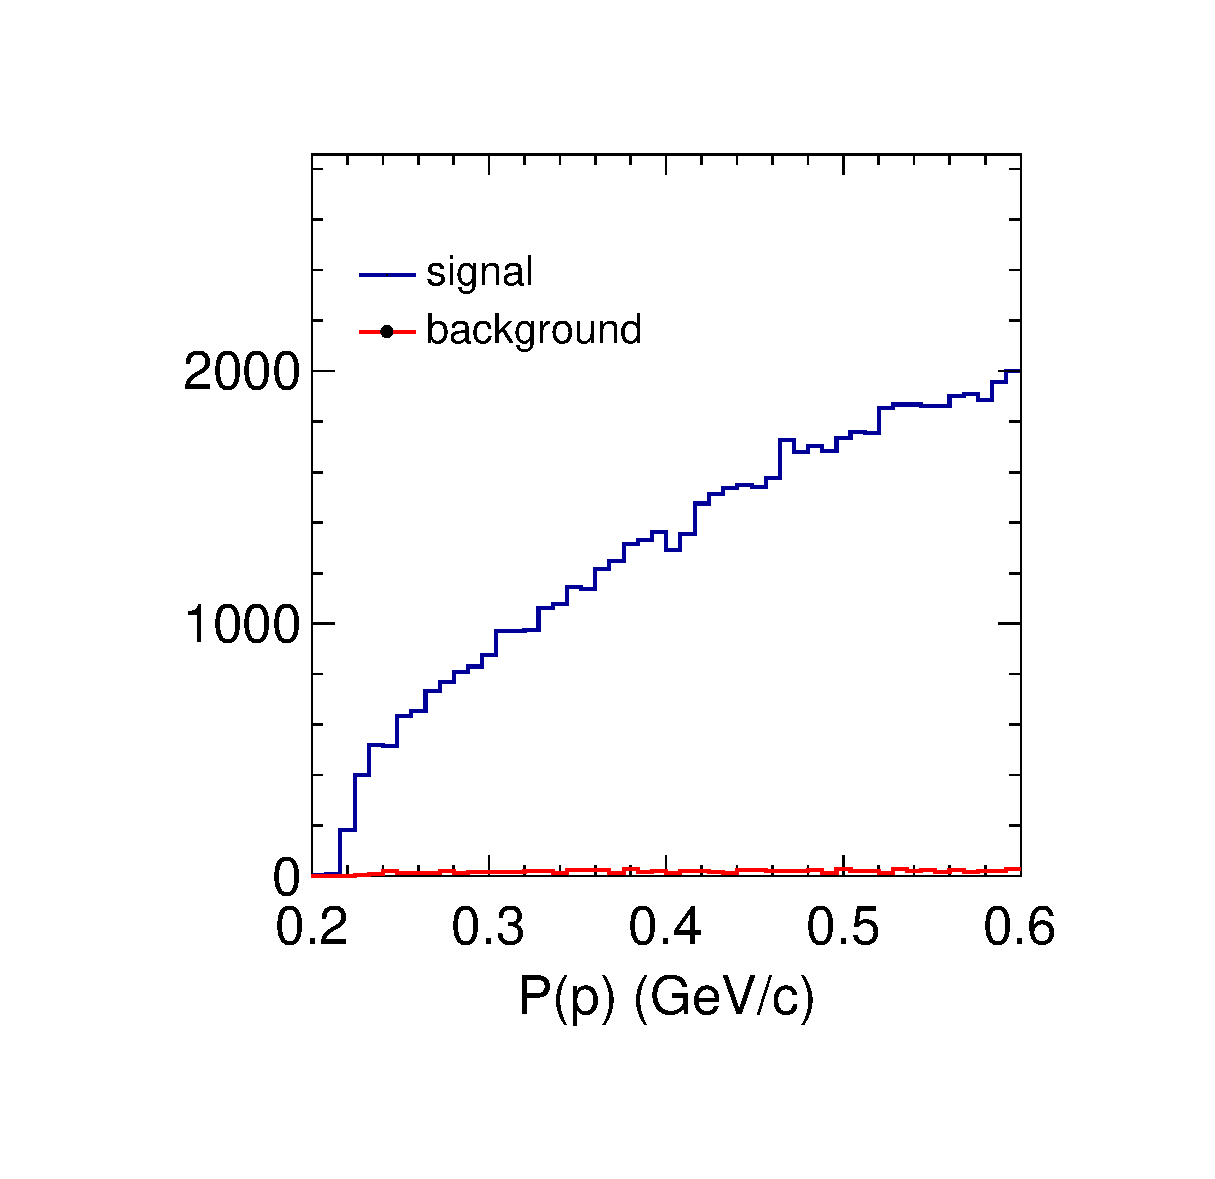
\includegraphics[width = 5 cm]{section/append/fig/momenta_pr_qqmc.eps}
    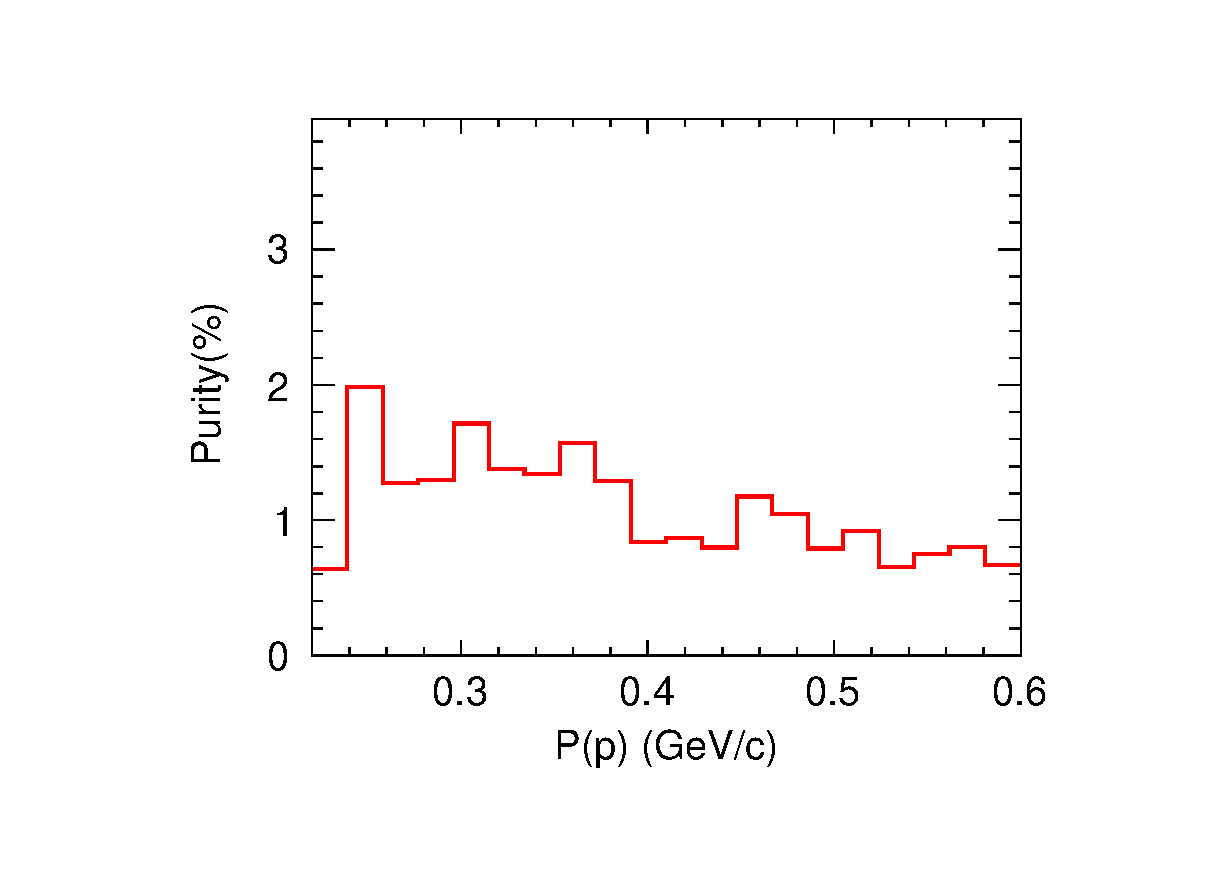
\includegraphics[width = 5 cm]{section/append/fig/Purity_pr_qqmc.eps}
    \caption{The momenta distribution for protons, and the red line
        shows the background level. Right figure shows th e purity of
    control sample based on cocktail MC sample.} 
    \label{Fig: bkg level for proton}
\end{figure}        

\subsubsection{PID efficiency}
The detail requirements of PID for proton and anti-proton are listed
following: 
\begin{itemize}
    \item use dEdx and TOF with correction information.
    \item $|\chi| < 9 $
    \item prob(p) $>$ 0,prob(p) $>$ prob(K) and prob(p) $>$ prob($\pi$)
\end{itemize}

To obtain the PID efficiency for proton (anti-proton), we fit to the
$MM^{2}$, which is defined as

\begin{equation} 
    MM^{2} = \left( E_{cms} - E_{\bar{p}} - E_{\pi^{+}} -
    E_{\pi^{-}} \right)^{2} - \left( - p_{\bar{p}} - p_{\pi^{+}} -
    p_{\pi^{-}} \right)^{2}
\end{equation}

We use the signal Monte Carlo line shape (MC truth matched) to model
the signal, and use the shape of $MM^{2}$ while 4-C kinematic
$\chi^{2}$ larger than 300 to model the background.  Since the PID
efficiency depends on the momentum of proton, we divide the momentum
into several bins with each bin width of 50 MeV$/c$. And we compare the
$cos\theta$ distribution data and MC for proton (anti-proton), Fig.
\ref{Fig: compare cost bewteen data and MC} shows MC can consist with
data very well, so we negelect the affection of the $cos \theta$ on the
PID efficiency. 

\begin{figure}
    \mbox{
        \begin{overpic}[width = 8 cm]{section/append/fig/Compare_cos_pr_data_Mc.eps}
            \put(75,75) {$(p)$}
        \end{overpic}
        \begin{overpic}[width = 8 cm]{section/append/fig/Compare_cos_antipr_data_Mc.eps}
            \put(75,75) {$(\bar{p})$}
        \end{overpic}
    }
    \caption{Compare the $cos\theta$ distribution between data and MC
    for proton and anti-proton}
    \label{Fig: compare cost bewteen data and MC}
\end{figure}
\subsubsection{The difference of PID efficiency between data and MC}

We fit the $MM^{2}$ spectroscopy in each bin shown in Fig.  \ref{Fig:
pass PID}, \ref{Fig: not pass PID}, and obtain the numbers of protons
pass or not pass the PID criteria, respectively. Then the differences
between data and MC are determined shown in Fig. \ref{Fig: difference
of PID efficiency} for the correction of the DT efficiency.  It's easy
to conclude that the statistics of the sample is too low to obtain more
accurate result on the difference between data and MC. We suggest the
Collection should collect some data at $E_{cm} = 3.097$ for systematic
study, because of the large cross section of $J/\psi$.

\begin{figure}[htbp]
    \mbox{
        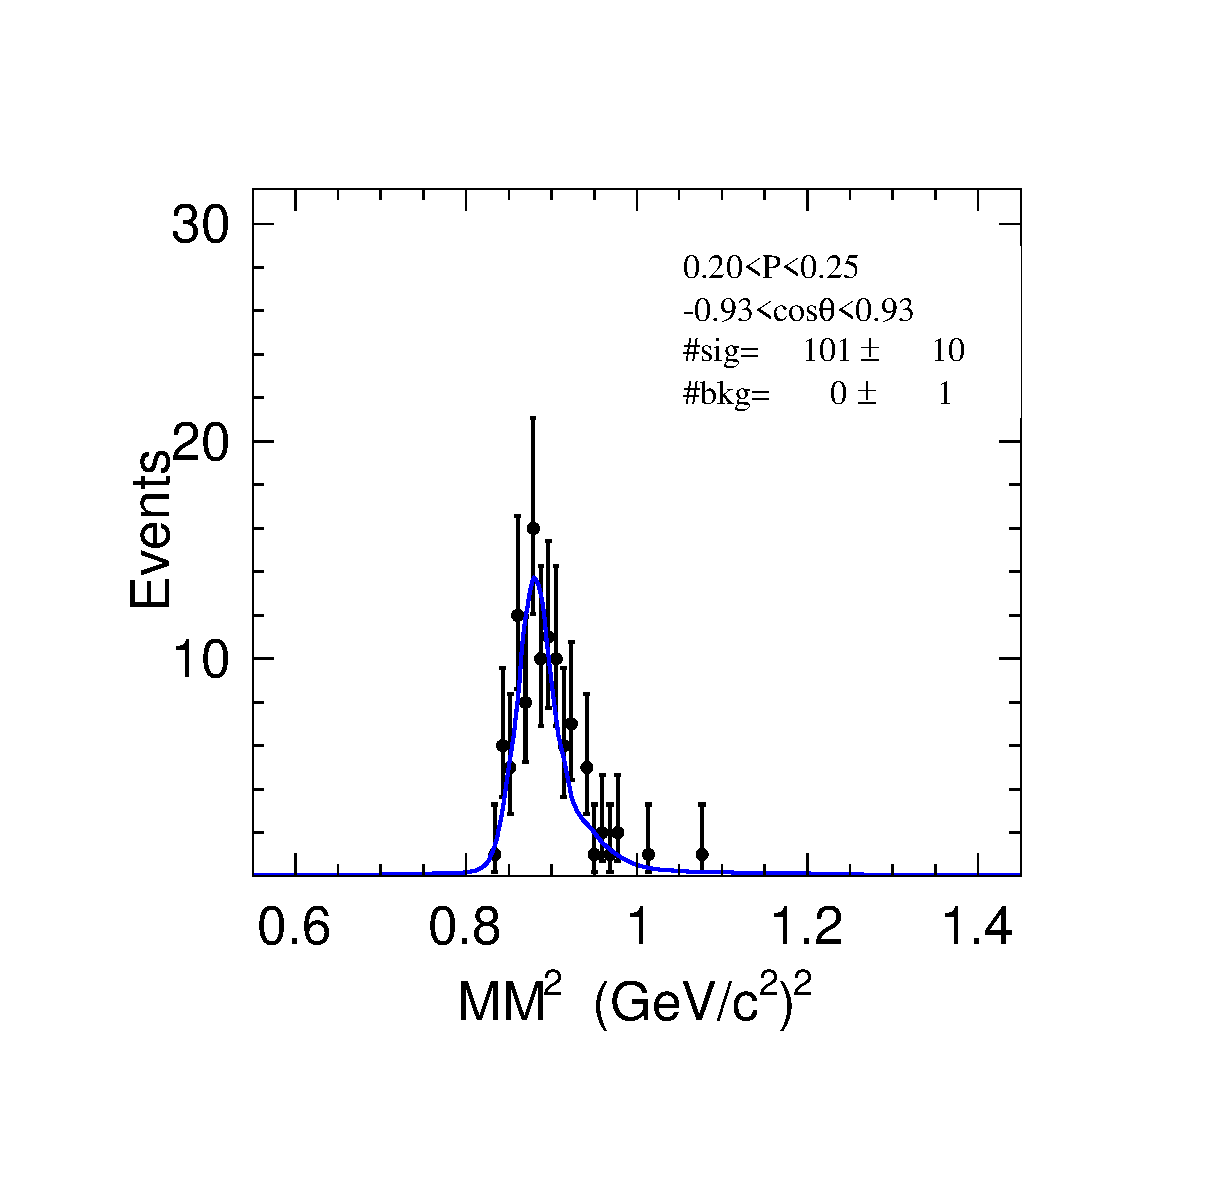
\includegraphics[width = 5 cm]{section/append/fig/Plot_MMSq_0_0_data.eps}  
        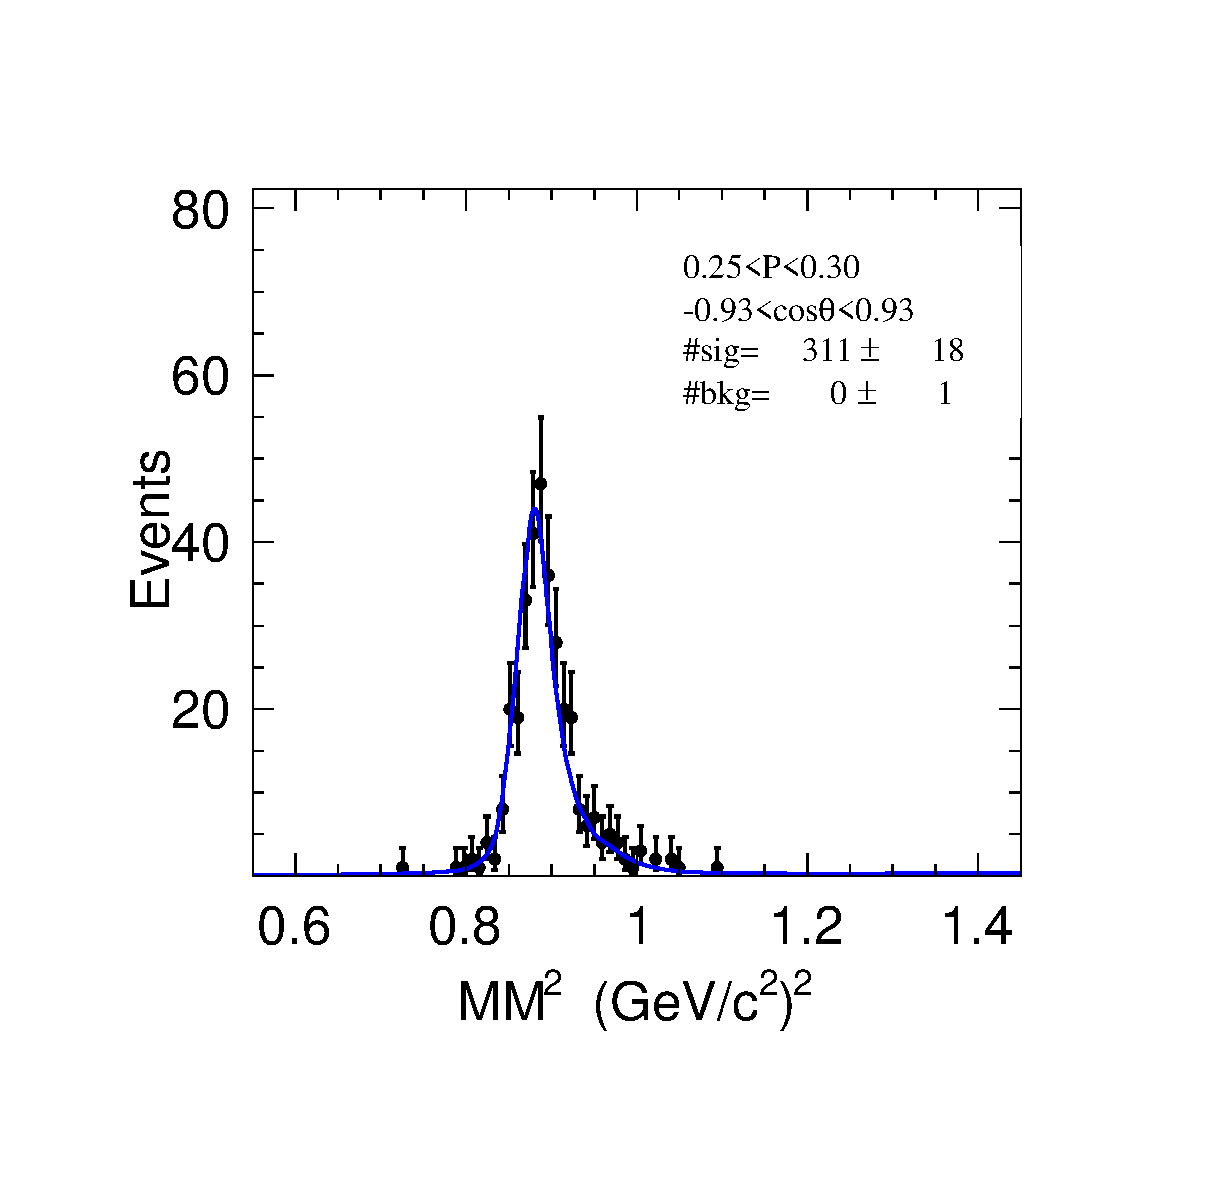
\includegraphics[width = 5 cm]{section/append/fig/Plot_MMSq_1_0_data.eps}
        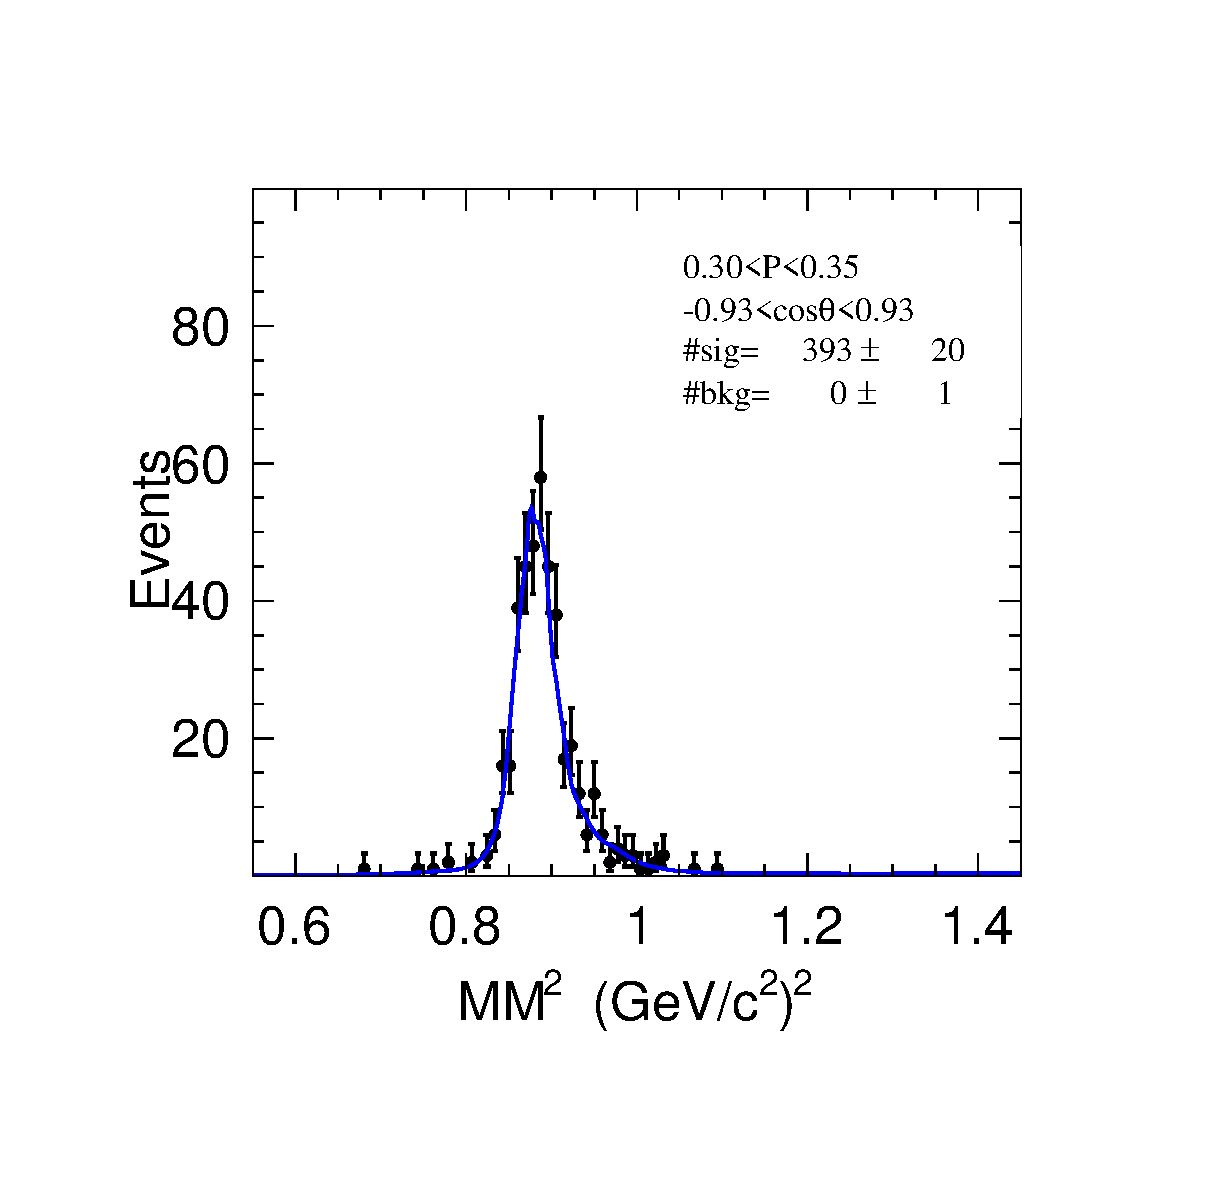
\includegraphics[width = 5 cm]{section/append/fig/Plot_MMSq_2_0_data.eps}       
    }
    \mbox{
        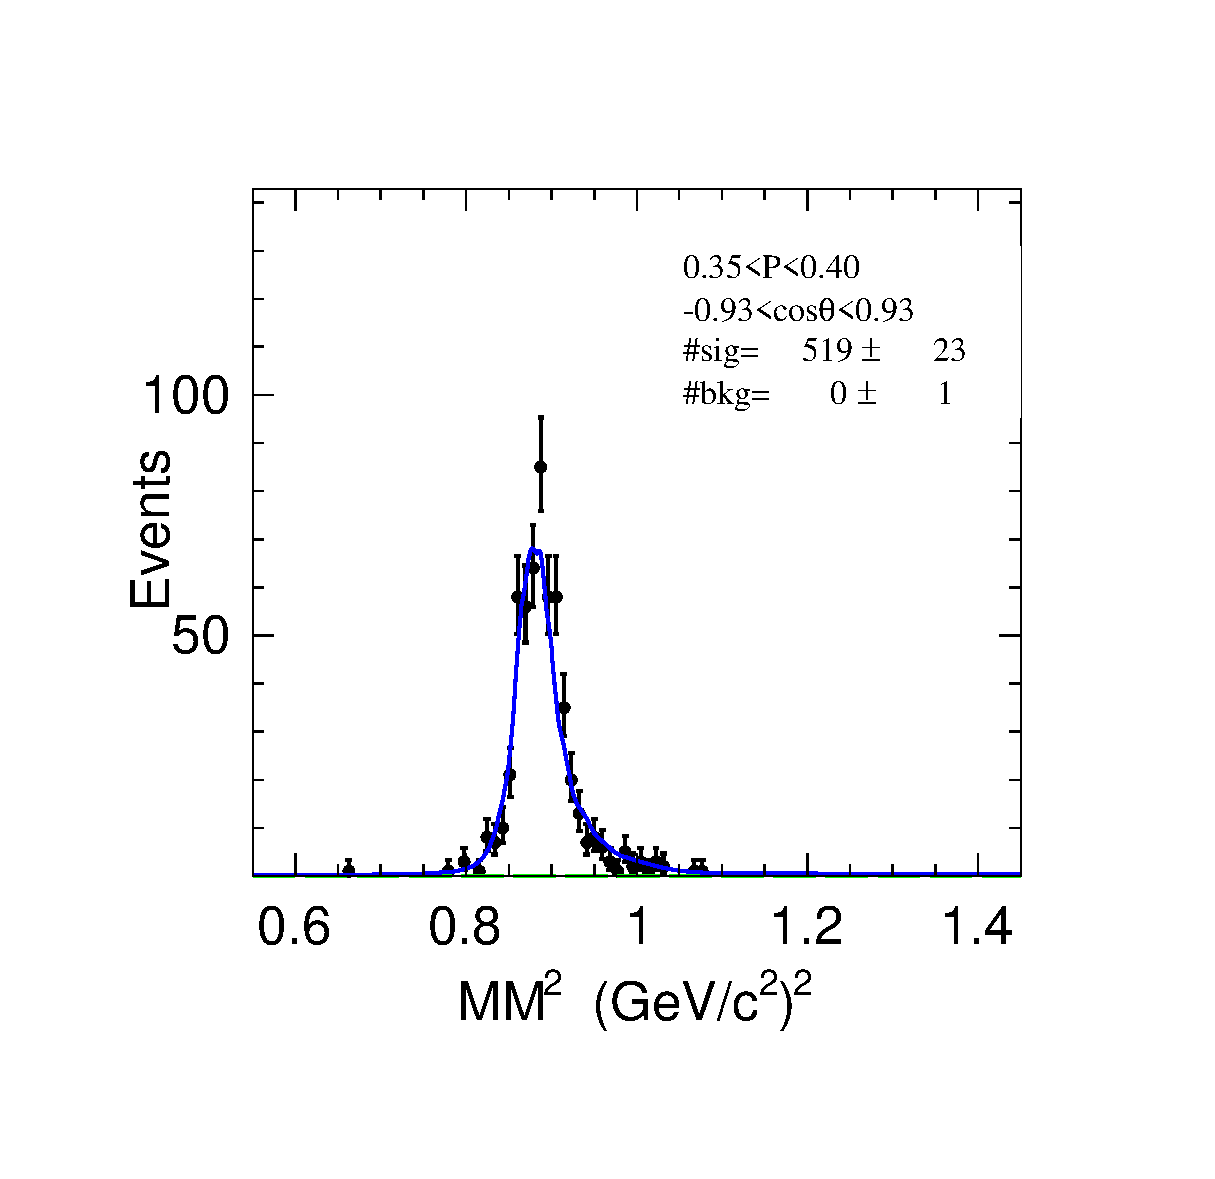
\includegraphics[width = 5 cm]{section/append/fig/Plot_MMSq_3_0_data.eps}  
        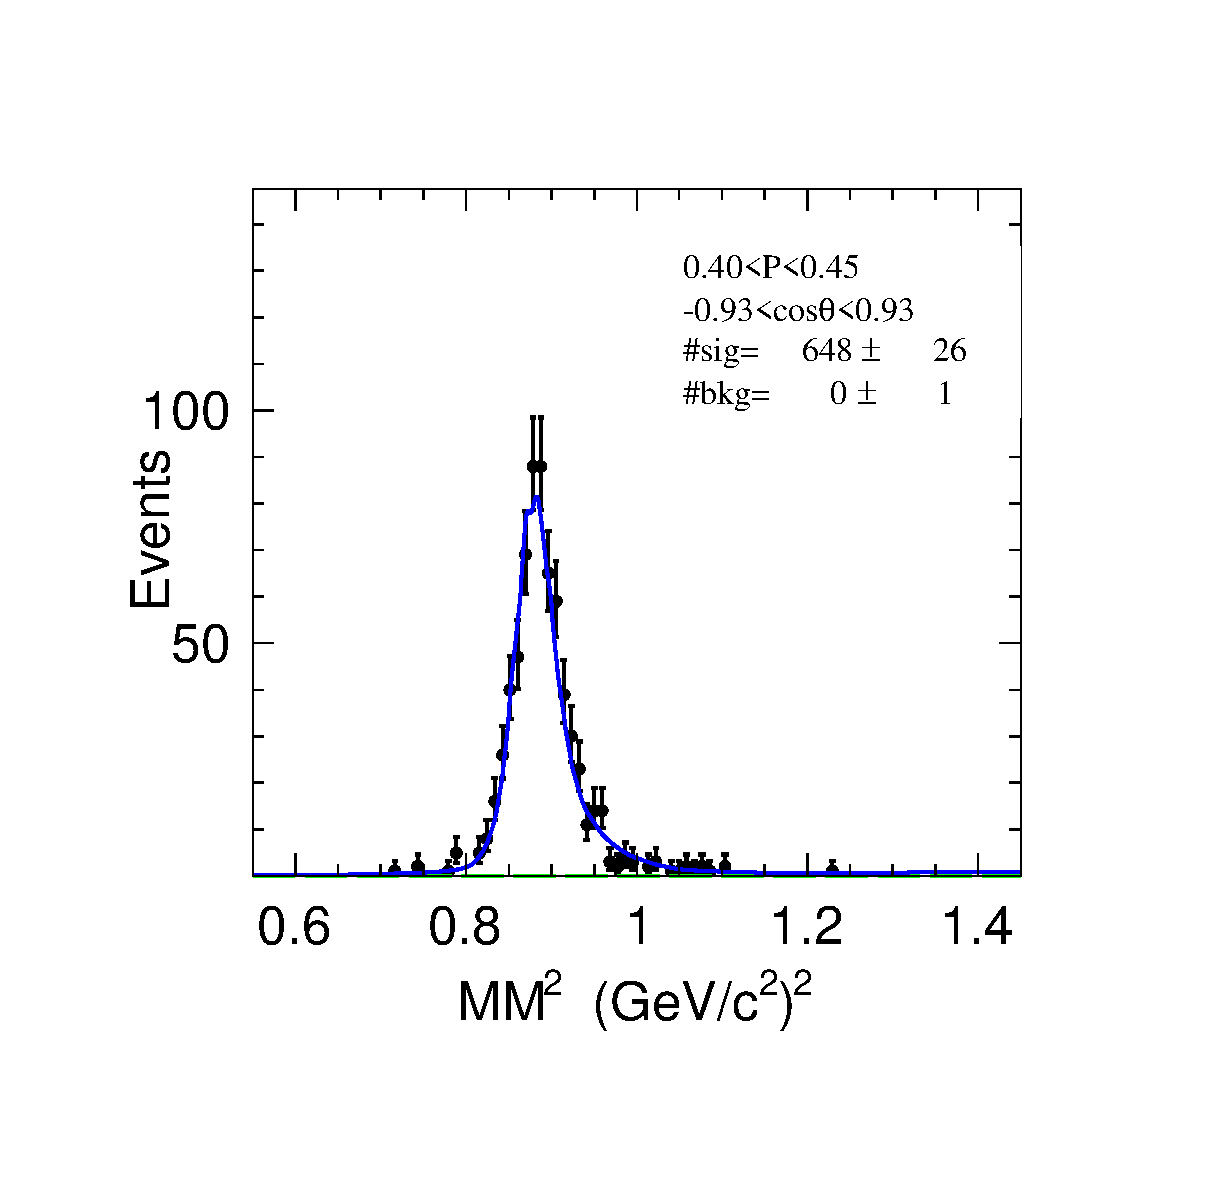
\includegraphics[width = 5 cm]{section/append/fig/Plot_MMSq_4_0_data.eps}
        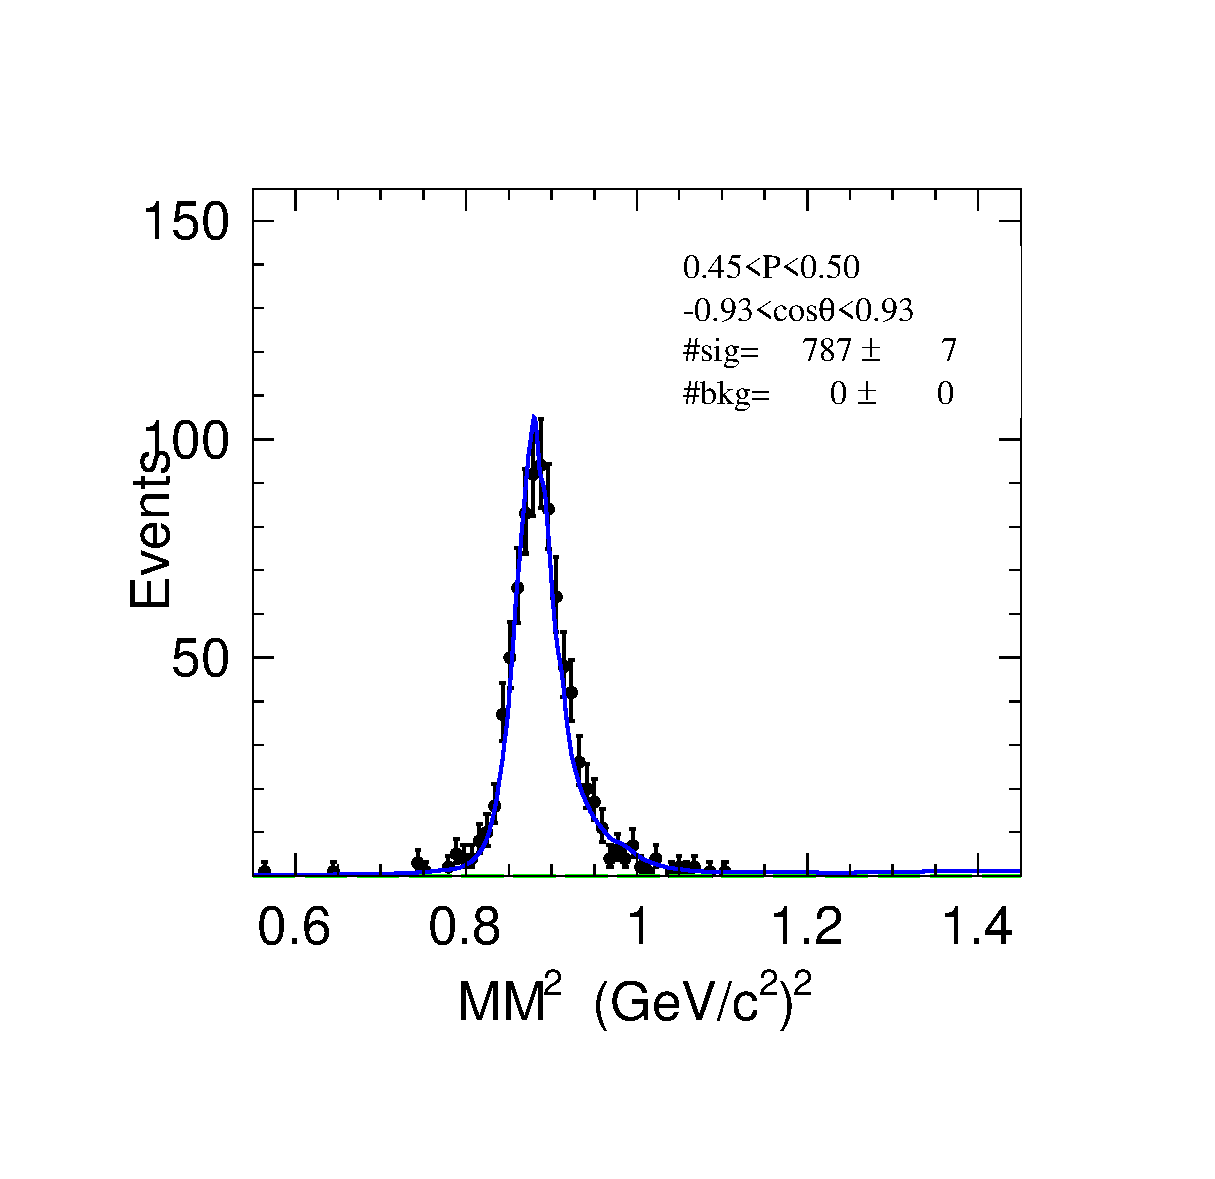
\includegraphics[width = 5 cm]{section/append/fig/Plot_MMSq_5_0_data.eps}       
    }
    \caption{The yields of proton passing the PID criteria in each bin.}
    \label{Fig: pass PID}
\end{figure}

\begin{figure}[htbp]
    \mbox{
        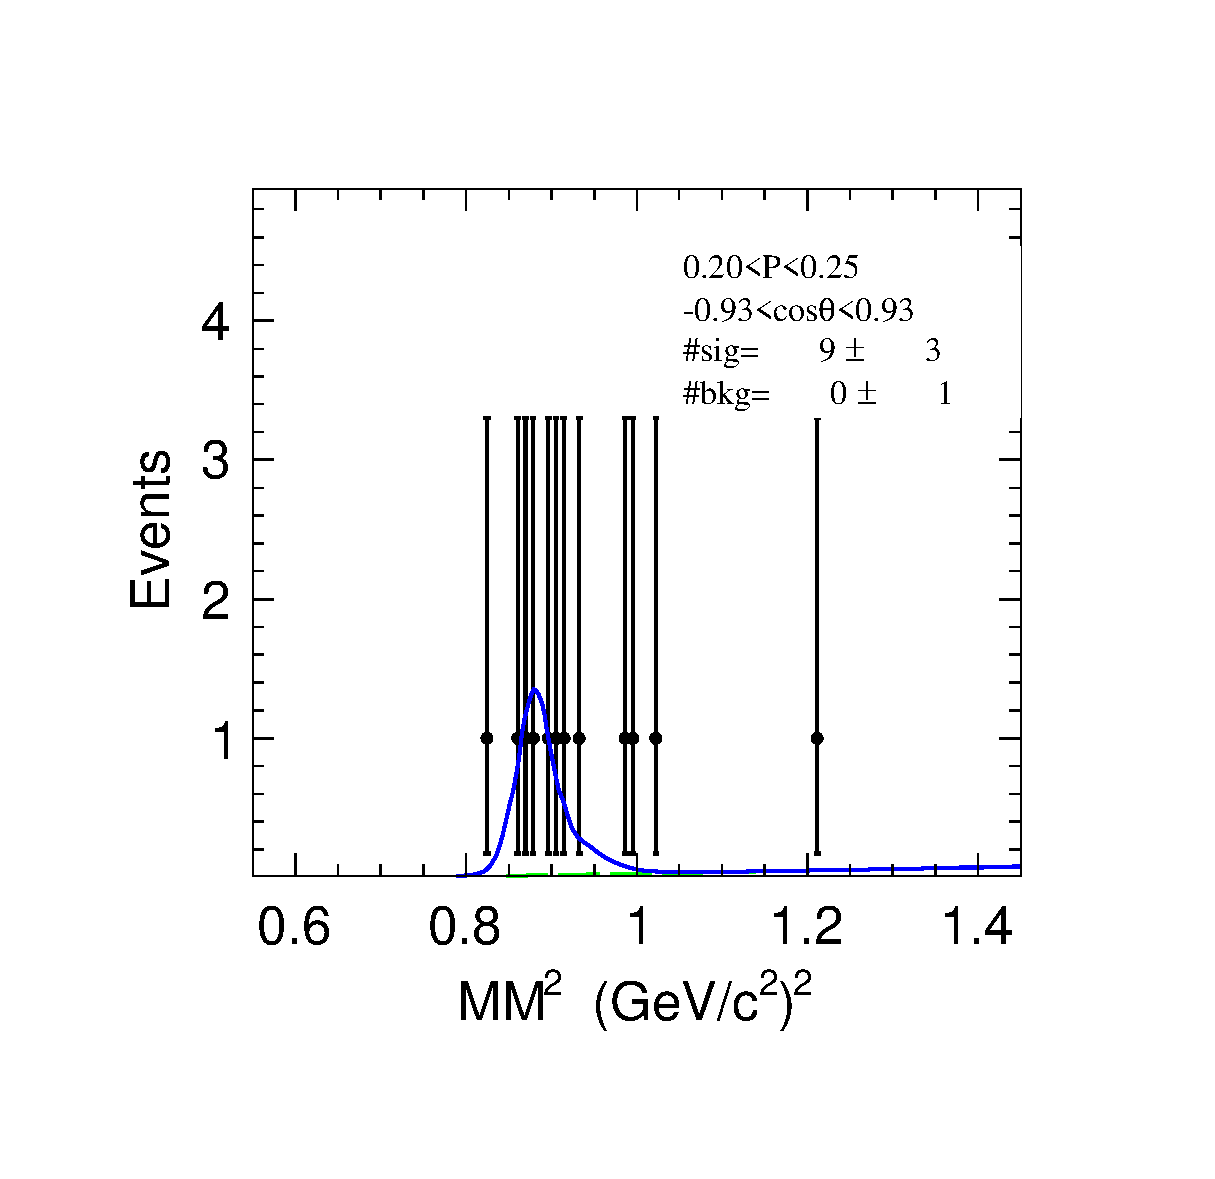
\includegraphics[width = 5 cm]{section/append/fig/Plot_MMSq_unpid_0_0_data.eps}  
        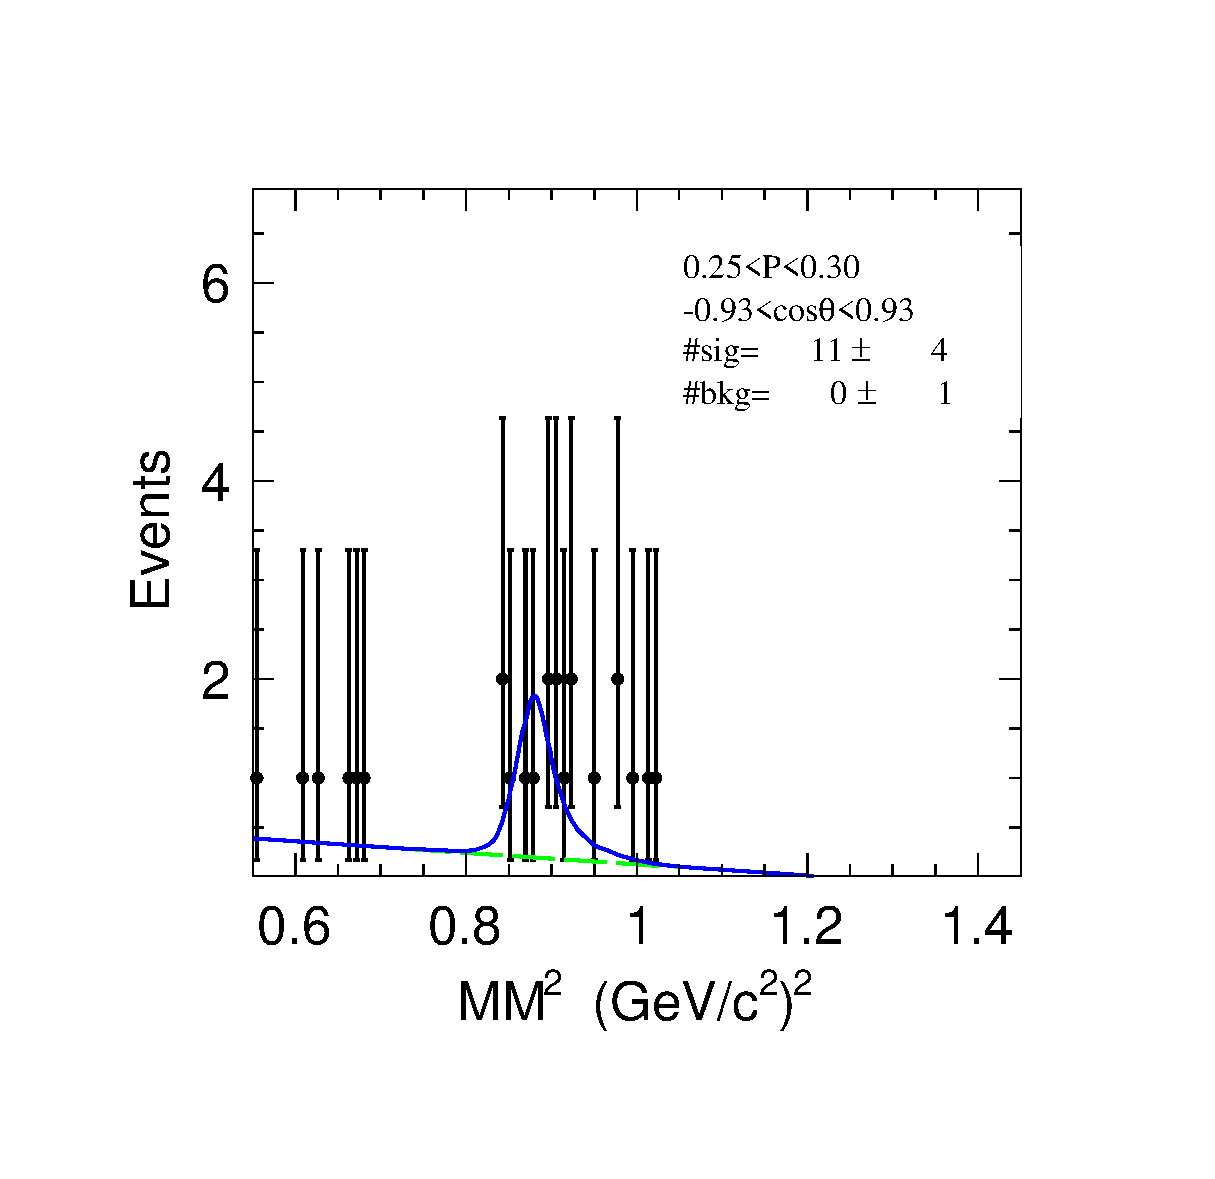
\includegraphics[width = 5 cm]{section/append/fig/Plot_MMSq_unpid_1_0_data.eps}
        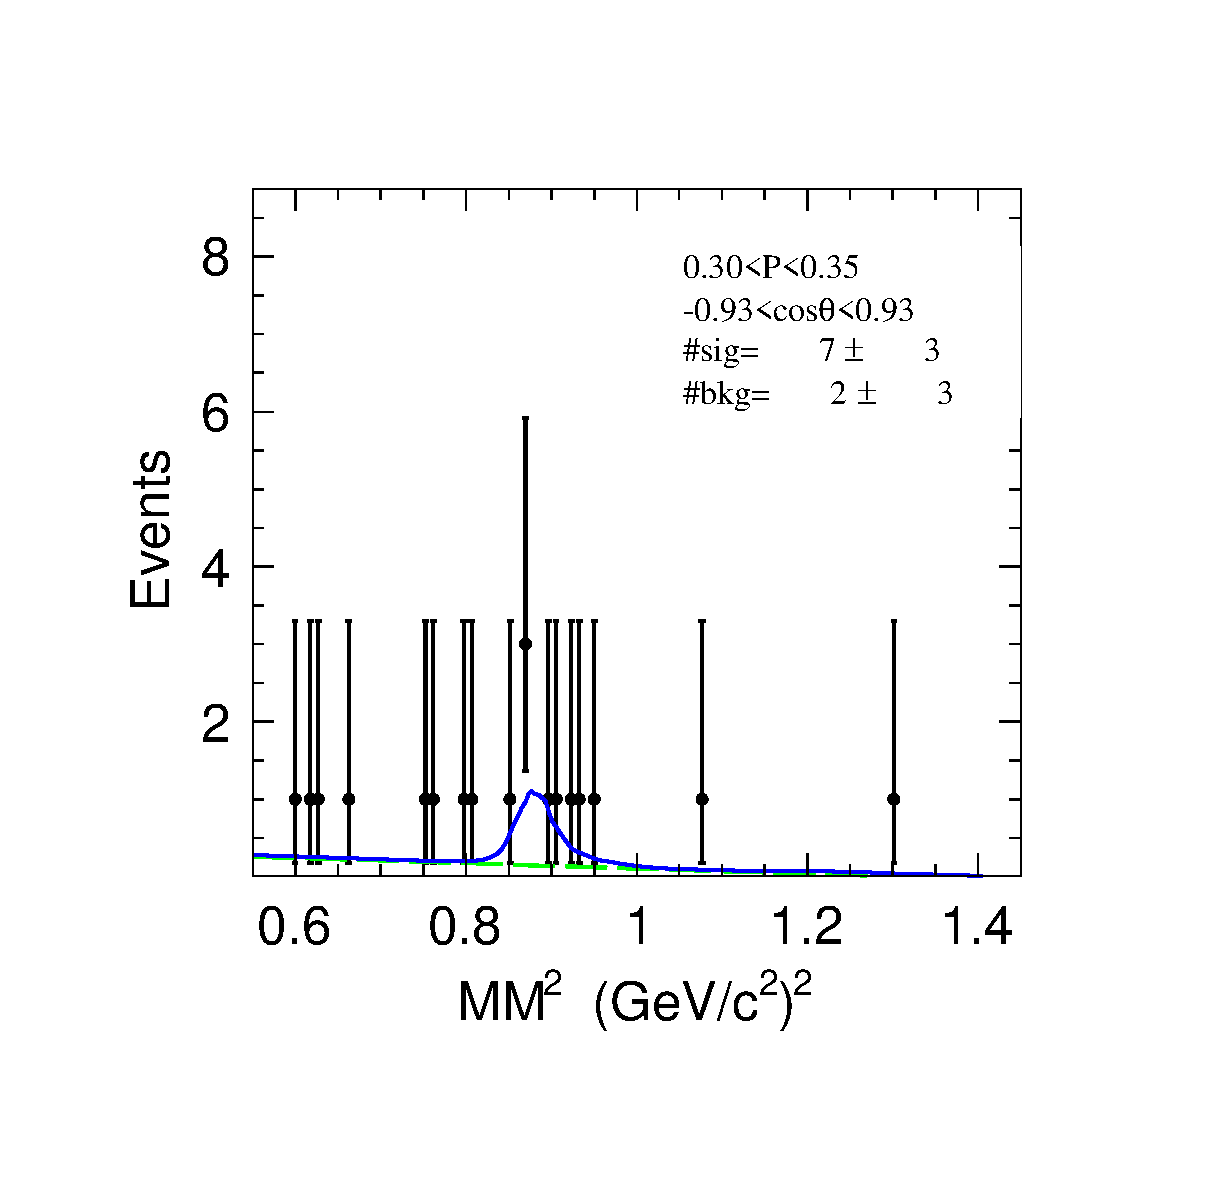
\includegraphics[width = 5 cm]{section/append/fig/Plot_MMSq_unpid_2_0_data.eps}       
    }
    \mbox{
        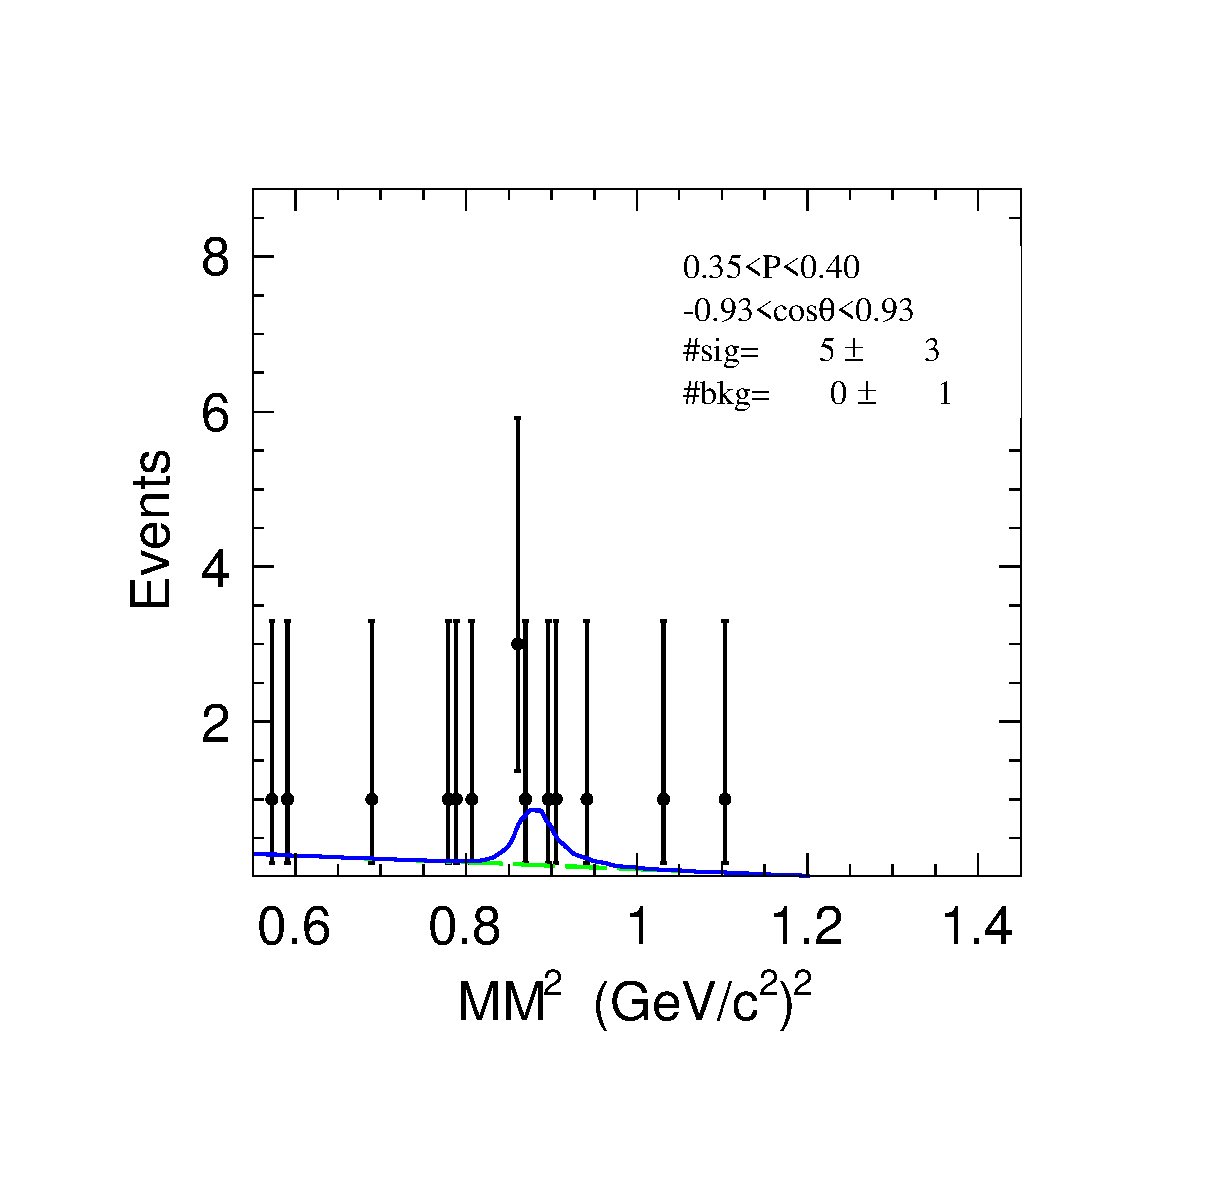
\includegraphics[width = 5 cm]{section/append/fig/Plot_MMSq_unpid_3_0_data.eps}  
        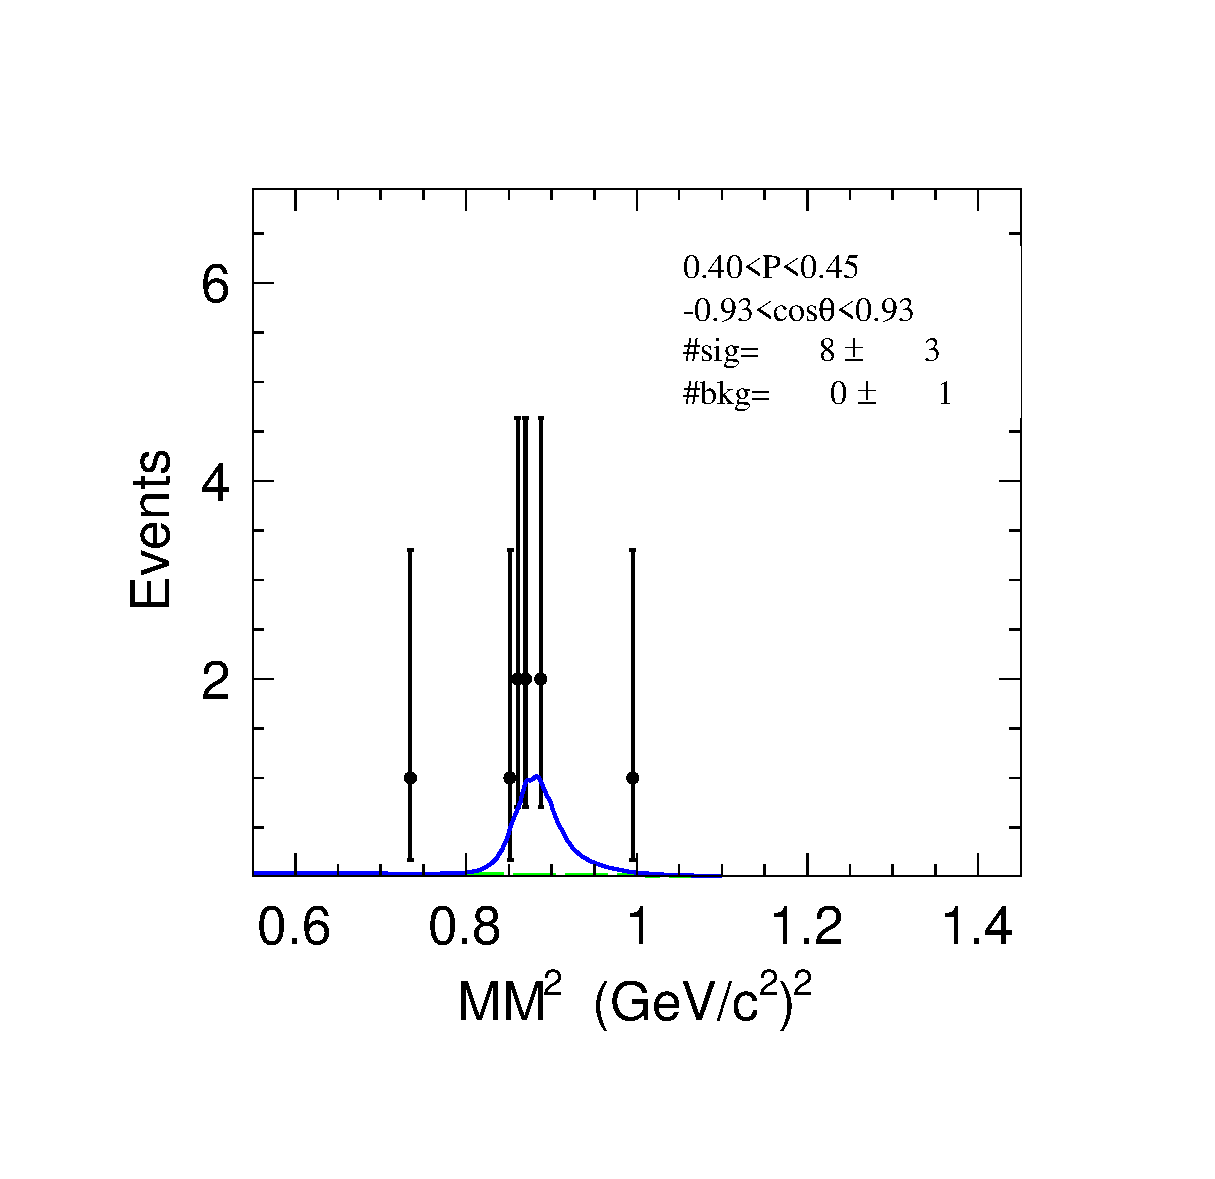
\includegraphics[width = 5 cm]{section/append/fig/Plot_MMSq_unpid_4_0_data.eps}
        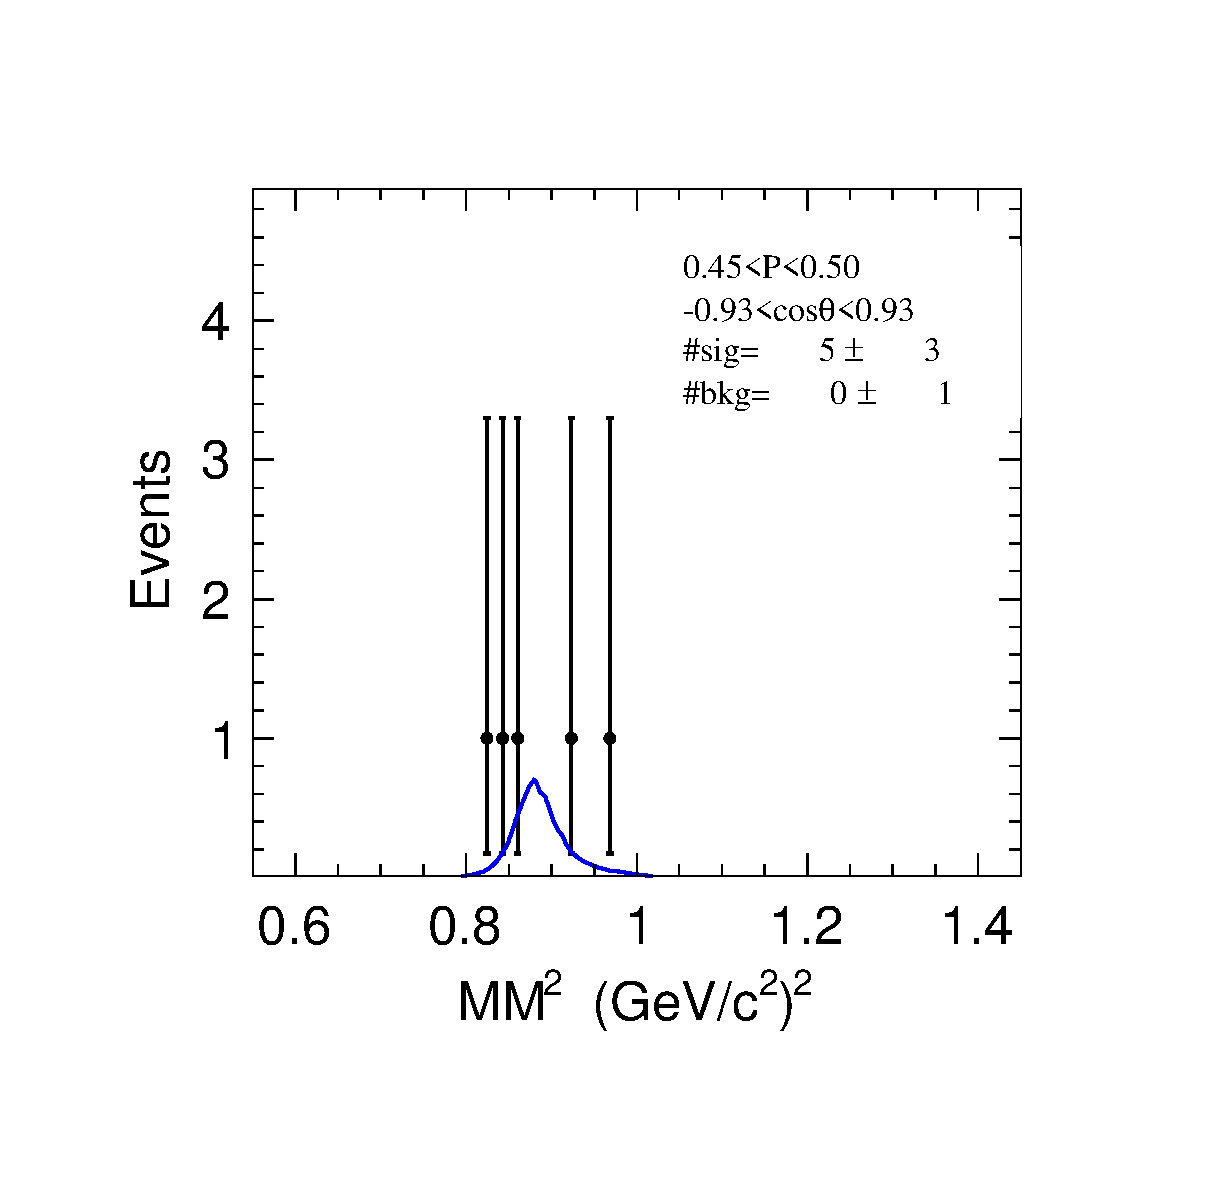
\includegraphics[width = 5 cm]{section/append/fig/Plot_MMSq_unpid_5_0_data.eps}       
    }
    \caption{The yields of proton failing to pass the PID criteria in each bin in data. The points with bars are data, blue solid lines are the sum of the fit functiond, and the red solid lines are the background shapes.}
    \label{Fig: not pass PID}
\end{figure}

\begin{figure}[htbp]
    \mbox{
        \begin{overpic}[width = 8 cm]{section/append/fig/Compare_eff_data_MC_pr.eps}     
            \put(75,75) {$(p)$}    
        \end{overpic}
        \begin{overpic}[width = 8 cm]{section/append/fig/Compare_eff_data_MC_antiPr.eps}     
            \put(75,75) {$(\bar{p})$}    
        \end{overpic}
    }
    \caption{The differences of PID efficiency between data and
        MC. The green and red points with error bars are efficiencies
    in MC and data, respectively.}
    \label{Fig: difference of PID efficiency}
\end{figure}

